\documentclass[a4paper, 12pt]{scrartcl}



\usepackage[utf8]{inputenc}

\usepackage[english]{babel}
\usepackage{amssymb}
\usepackage[T1]{fontenc}
\usepackage{mathtools}
\usepackage{amsmath}
\usepackage{ntheorem}
\usepackage{bbm}
\usepackage{dsfont}
\usepackage{color}
\usepackage{slashed}
\usepackage{hyperref}
\usepackage{graphicx} 
\usepackage{subcaption}
\usepackage{bm}
\usepackage{mathabx}
\usepackage{multirow}
\usepackage{float}
\usepackage{changepage}
\usepackage{mwe}
\begin{document}
\begin{titlepage}
	\centering
	{\scshape\LARGE University of Tübingen \par}
	\vspace{2cm}
	{\huge\bfseries Solar cell \par}
	\vspace{2cm}
	{\Large \scshape Blockpraktikum 2021} \par
	\vspace{2cm}
	{\Large  First Version} \par
	\vspace{2cm}
	{\Large\itshape \underline{Christian Gommeringer}\space \space \underline{Matthias Gatter}\space \space \underline{Jonathan Witte}\space \space \underline{Eduard Heidt}\space \space \underline{David Schütz}\par}
	\vfill 
	{\large overlooked by Tao Wei}
	\vfill

	{\large \today\par}
\end{titlepage}
\newpage 
\tableofcontents 

\newpage
\section{Introduction} 
A solar cell converts photonenergy into a electrical energy which is usable in form of a electric current. In this experiment we analyse the behavior of a solar cell in diffrent views of physical describtion. First we talk about the theoretical fundamentals to make us clear about the physical relations. After that we describe the experiment and it´s execution. All in all we then hand over to the analysis of our measurments and present our results. 

\section{Theoretical Fundamentals}
\subsection{Questions} 
What is the diffrence between metals, insulators and semiconductors? 
\newline 
\newline 
Answer: An insulator has in band theory a unoccupied conduction band cause of the big band gap. So in low and high temperatures are only a few electrons which are thermally stimulated from the valence band into the conduction band. Semiconductors have a much smaller band gap, which makes it possible for electrons by thermal stimulation to get up to the conduction band. The band gap is moveable. A semiconductor has a low conductivity in room temperature and the conductivity can be increased by heating the semi conductor. In metals the band gap is very small or the valence band and the conduction band are overlapping. This makes a metal a good conductor by room temperature. 
\newline 
\newline 
What is the role of electrons, holes, and doping in semiconductor’s physics? 
\newline 
\newline 
Answer: If a elektron is thermally stimulated in the valence band, it jumps over the the conduction band. So there is now a hole in the valence band which can be filled, for example a atom and at this point we have doting. There are two types of doting, n-doting where you bring in an atom which one of the electrons is weak bounded an can easily stimulated into the conduction band, such atoms are called electron donators and on the other side we have p-doting, where the atom has an electron missing and can take electrons from the conduction band in their boundness and bring them into the valence band, such atoms are called electron acceptors. 
\newline 
\newline 
How is a semiconducting diode build up? What is the diode equation and how does the
IV curve of a diode looks like?
\newline 
\newline 
Answer: The base of a semiconducting diode is a p-n-doted semiconducting crystal or a metal-semiconductor-transition (Schottky Diode). The conductivity of such a transition depends on the polarity of the operating voltage on the anode (p-doted) and cathode (n-doted), also it depends on the current direction. The p-n-transition (grey zone) is a zone where charges can move freely, cause positive charges (defect electrons or holes) of the p-doted crystal and negative charges (free electrons) of the n-doted crystal are diffusing on the other side of the p-n-transition and are disapearing cause of recombination. The origin of the charges are doted atoms which are fixed in position and they are forming as ions a space charge, which electrostatic field is building space charge zone which keeps the to sides seperated and stops more recombination. Over the whole space charge zone is forming a diffusing voltage. The diffusing voltage can through a outside applied voltage be compensated, then the p-n-transition can be conductive or be strengthened , then it keeps blocked.
\newline 
\hspace*{+3cm}
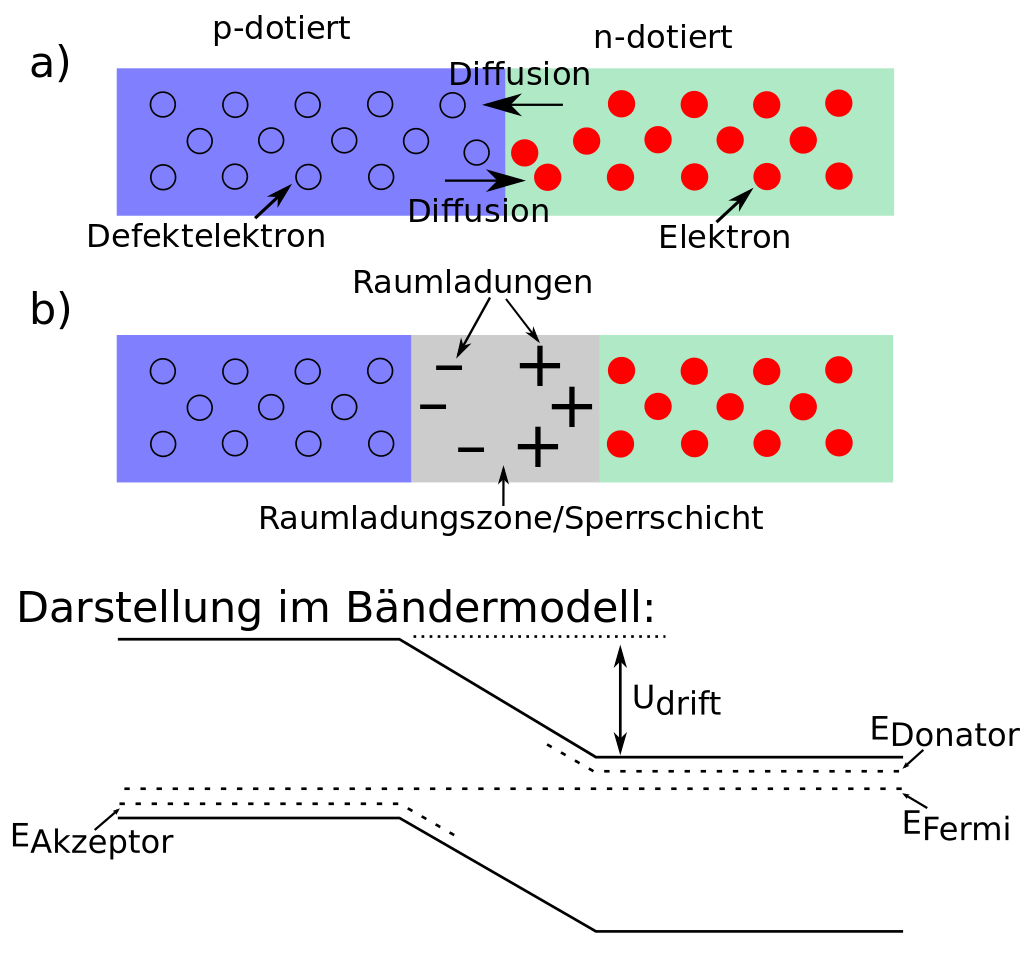
\includegraphics[scale=0.25]{szpic1}
\newline 
\textbf{Illustration 1:} p-n-transition, source:\space \url{https://de.wikipedia.org/wiki/Diode#/media/Datei:Sperrschicht.svg}
\newline
\hspace*{+3cm}
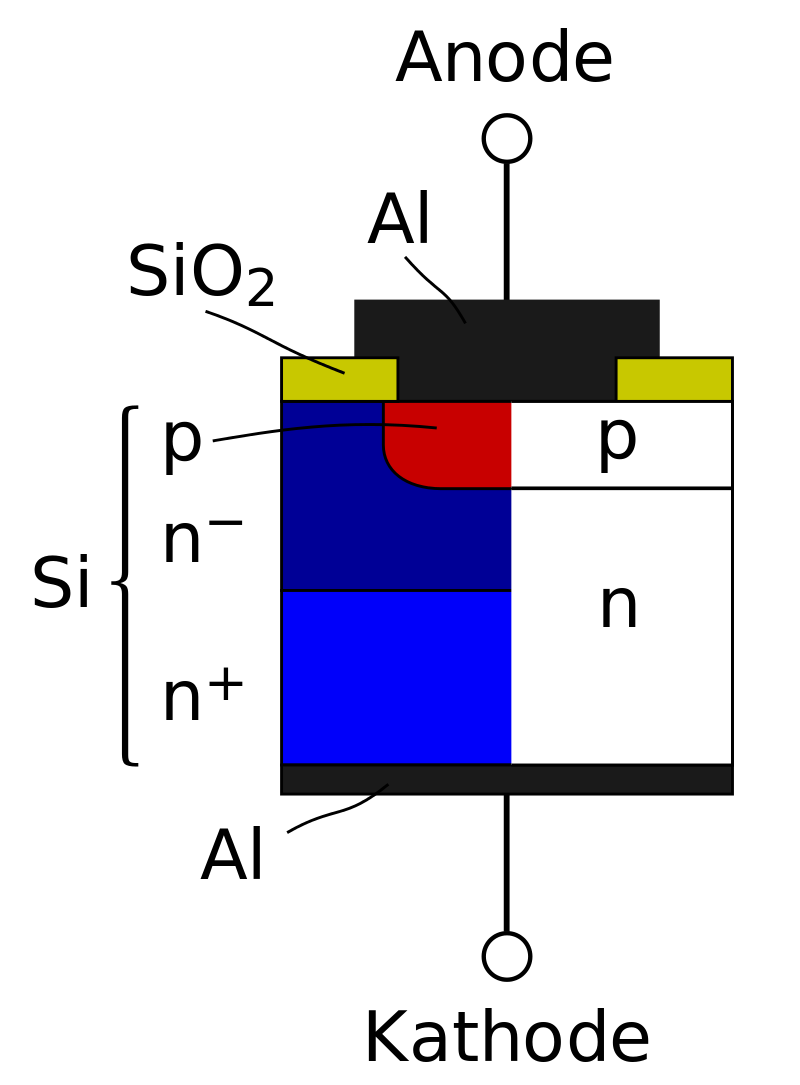
\includegraphics[scale=0.18]{szpic2}
\newline 
\textbf{Illustration 2:} Schematic example of a p-n-diode: source: \url{https://de.wikipedia.org/wiki/Diode#/media/Datei:Pn-Diode-Aufbau.svg}
\newline 
The diode equation is given by 
\begin{align}
I_\textrm{D} = I_\textrm{S}(T) \left( \exp \left( \frac{ U_\textrm{F}}{n U_\textrm{T}} -1 \right) \right) 
\end{align}
where $I_\textrm{D}$ is the diode current, $I_\textrm{S}(T)$ the temperature dependent saturation current, $U_\textrm{F}$ the forward voltage , $n$ the emission coefficient, $U_\textrm{T} = \frac{k_\textrm{B} T}{e}$ the temperature voltage, $k_\textrm{B}$ the boltzmann constant, $e$ the elementary charge. We also take a look at the characteristic curve of a diode current. 
\newline 
\hspace*{+4cm}
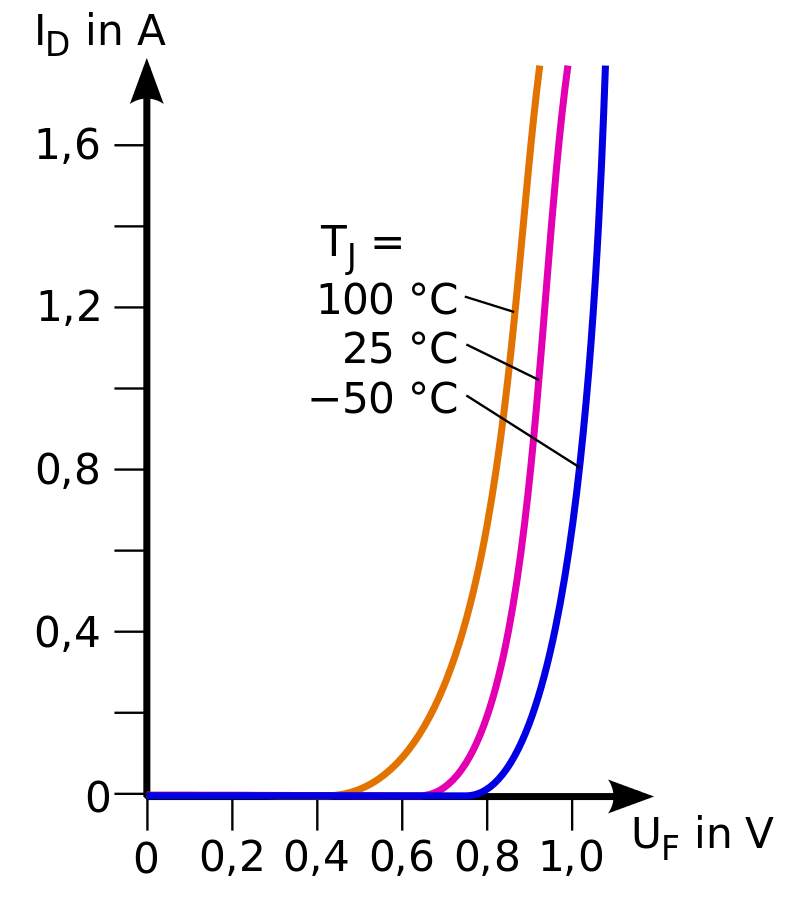
\includegraphics[scale=0.2]{szpic3}
\newline 
\textbf{Illustration 3:} Characteristic curve of the diode, source: \url{https://de.wikipedia.org/wiki/Shockley-Gleichung#/media/Datei:Dioden-Kennlinie_1N4001.svg}
\newline 
\newline 
What ist the internal photoelectric effect and what is the photovoltaic effect? 
\newline 
\newline How does the IV-curve of a solar cell looks like? How can the most important cell parameters be extracted from the IV curve, i.e., the short circuit current, the open circuit
voltage, the maximum power point, the fill factor, the efficiency, the parallel resistance
and the serial resistance?
\newline 
\newline 
These two Questions will be later discussed and answered. 
\subsection{p-n-Transition of a diode}
Many solar types are made of the semiconductor material silicon. A crystal silicon solar cell is made of p-doted silicon-layer (base) which is in contact with a n-doted silicon-layer (emitter). In the contact zone between this two layers is forming the p-n-transition, which determines the physics of the solar cell. Cause of the concentration gradient of the charges in the contact zone, the holes are diffusing out of the p-zone into the n-zone and conversely electrons from the n-zone into the p-zone. In the p-zone are staying negative ionised acceptors and in the n-zone are staying positive ionised donators as fixed space charge. The space charge with diffent polarity on both sides of the interface leads to a electric field, thats forming a field current against the direction of the diffusing current which leads to a compensation. 
\subsection{Internal photoelectric effect}
If light shines on a solar cell, photons with energy greater or equal the band gap of the semiconductor material are getting absorbed. A absorbed photon leads to that a bound electron in the valence band is getting thermally stimulated and jumps to a niveau of the conduction band of the semiconductor. Together with to hole in the valence band they form a moveable electron-hole-pair. 
\newline 
\hspace*{+6cm}
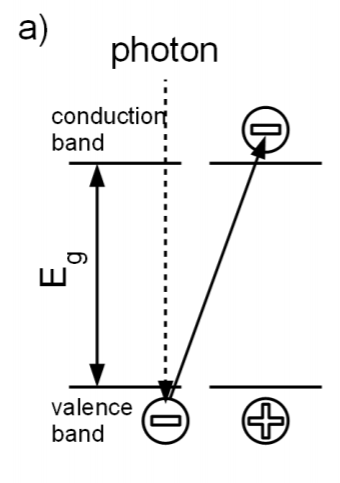
\includegraphics[scale=0.6]{szpic4}
\newline 
\textbf{Illustration 4a:} Schematics of the internal photoelectric effect. Source: experiment instruction
\subsection{Photovoltaic effect} 
Gets a photon in the space charge zone absorbed of the solar cell, it equalizes the electric field around the electron-hole-pair. The electron moves into n-zone und the hole into the direction of the p-zone. Gets the electron-hole-pair formed beyond the space charge region, so it cans by thermal motion diffuse into the space charge region. The electrons in the p-zone an the holes in the n-zone are getting accelerated onto the opposing side by the electric field of the space charge zone. Together the charges whiche are formed in the contact region , they form the photo current $I_\textrm{ph}$. Electrons in the p-zone are moving to the n-zone and the holes are moving from the n-zone to the p-zone. The p-side now gets positively charged and the n-side negatively, the potential diffrence can be tapped as no-load voltage. This process of light induced charge segregation at the p-n-transition of the diode is called photovoltaic effect.
\newline
\hspace*{+4cm} 
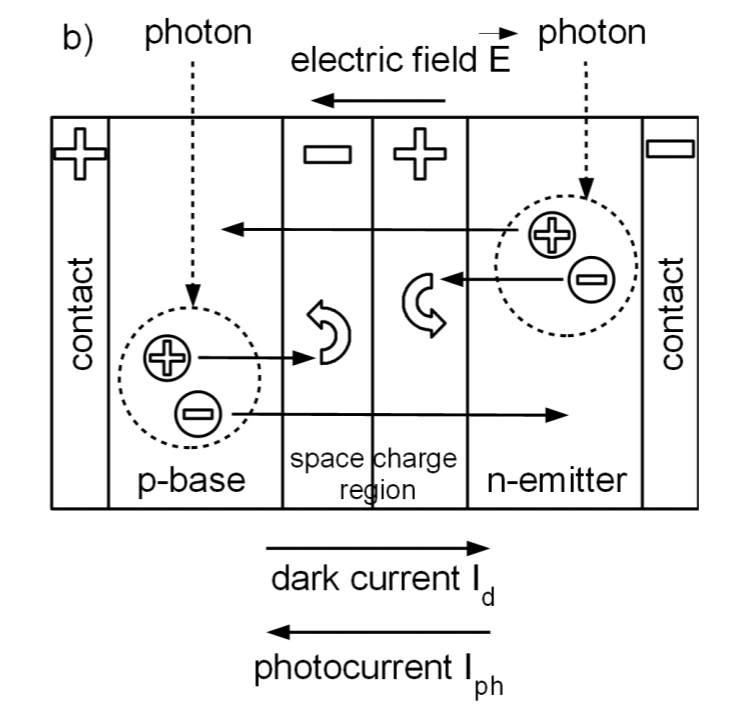
\includegraphics[scale=0.6]{szpic4b}
\newline
\textbf{Illustration 4b:} Schematics of the photovoltaic effect. Source: experiment instruction 
\newline 
\newline 
\subsection{One-Diode-Model}
In the following we derive the characteristic I-V-line of the solar cell. Every contribution of the output current $I$ can be illustrated by a equivalent circuit diagram of a real solar cell. 
\newline 
\hspace*{+4cm}
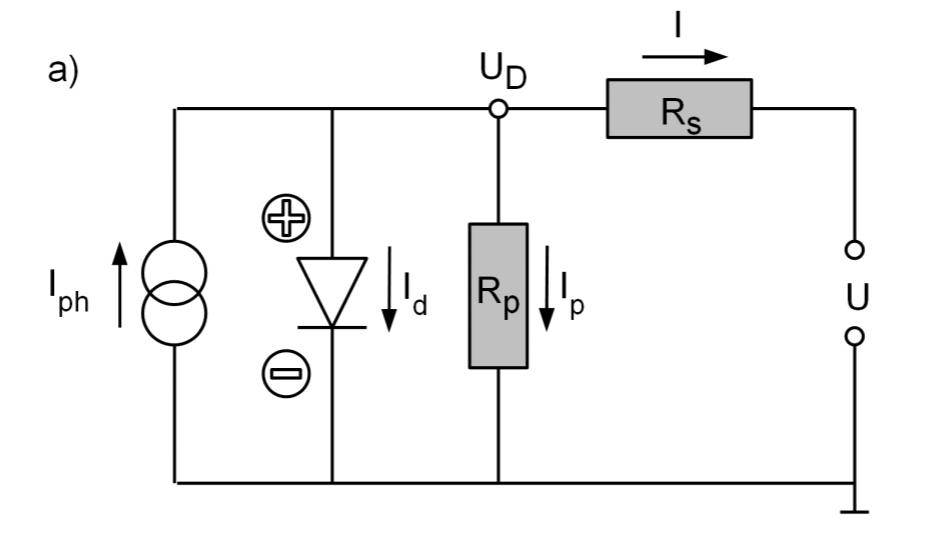
\includegraphics[scale=0.5]{szpic5a}
\newline 
\textbf{Illustration 5a:} equivalent circuit diagram, source: experiment instruction 
\newline 
The solar cell let itself be understood as parallel circuit of a current source, a forward poled diode, and of a parallel resistance $R_\textrm{p}$. The drawn current source delivers the constant photo current $I_\textrm{ph}$. The photo current $I_\textrm{ph}$ gets reduced through the diode current $I_\textrm{d}$ , through the current $I_\textrm{p}$ and through the parallel resistance $R_\textrm{p}$. The serial resistance reduces the output current and the tapped voltage.A unlit solar cell behaves like a diode cause of the p-n-transition. For a ideal diode is the IV-curve given by the diode equation
\begin{align}
I_\textrm{d}(U_\textrm{D}) = I_0 \left[ \exp \left( \frac{e U_\textrm{D}}{nk_\textrm{B}T}\right) -1 \right]
\end{align}
where $I_\textrm{d}$ is the dark current, $I_0$ the saturation current, $U_\textrm{D}$ the voltage drop over the diode, $T$ the cell temperature. The diode factor $n$ is approximatley one. $n \approx 1$. The saturation current $I_0$ gets calculated by the diffusion coefficients, the diffusion lengths for electrons and holes, the donator- and activator concentration and the intrinsic charge carrier density leads to a temperature dependence 
\begin{align}
I_0(T) \propto T^s \exp \left( - \frac{E_g}{k_B T} \right) 
\end{align}
where $E_g$ is the band gap energy and $s$ a material dependent exponent ($s=0$ for silicon). The IV-curve of an ideal solar cell is than given through 
\begin{align}
&\ I_\textrm{D}(U_\textrm{D}) = I_\textrm{ph} - I_\textrm{d}(U_\textrm{D})
\\ &\ I_\textrm{D}(U_\textrm{D}) = I_\textrm{ph} - I_0 \left[ \exp \left( \frac{e U_\textrm{D}}{nk_\textrm{B}T}\right) -1 \right]
\end{align}
Photo current and dark current are running in opposing directions, where the dark current runs from p-zone to n-zone, like a forward poled diode. For a real solar cell we have to consider the parallel resistance $R_\textrm{p}$ and the serial resistance $R_\textrm{s}$. With $R_\textrm{p} = U_\textrm{D}/ I_\textrm{P}$ and $R_\textrm{s}= (U_\textrm{D}-U)/I$ it follows
\begin{align}
&\ I(U_\textrm{D}) = I_\textrm{ph} -I_\textrm{d}(U_\textrm{D}) -I_\textrm{p}(U_\textrm{D}) \\ &\ 
I(U) = I_\textrm{ph}-I_0 \left[ \exp \left( \frac{e(U+IR_\textrm{s})}{nk_\textrm{B}T} -1 \right) \right] - \frac{U +IR_\textrm{s}}{R_\textrm{p}}
\end{align}
with output current $I$ and output voltage $U$, with can be tapped at the solar cell. 
\subsection{Cell parameters}
Out of the IV-curves it is possible to calculate the cell parameters approximately. 
\newline 
\hspace*{+3cm}
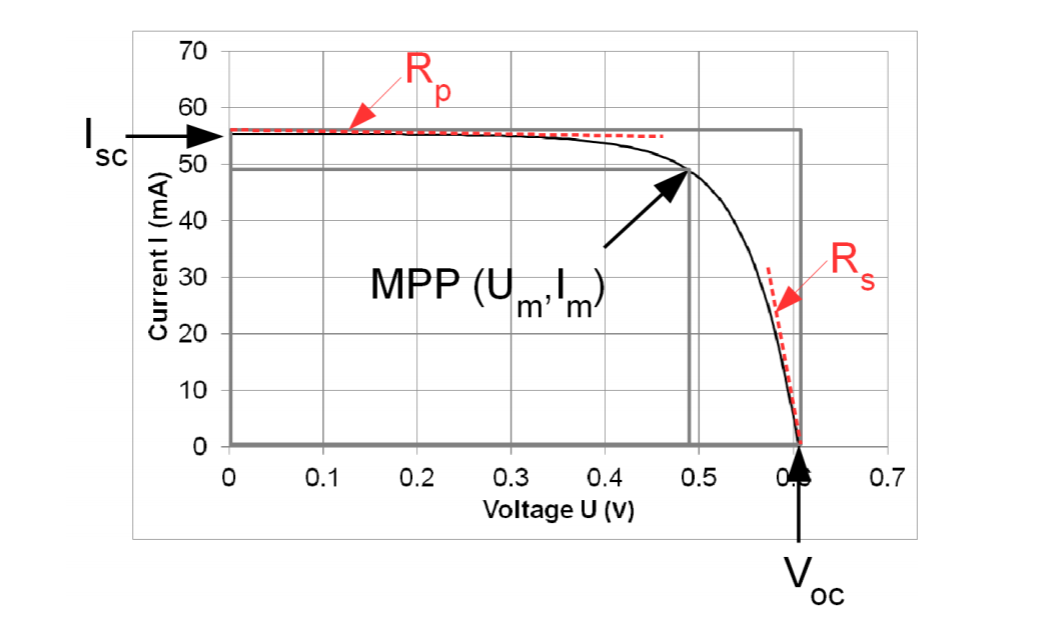
\includegraphics[scale=0.5]{szpic62}
\newline 
\textbf{Illustration 6:} Determination of cell parameters, source: experiment instruction
\newline 
\newpage
The parameters can be extracted of certain characteristics of the the I-U curves, often in approximated way. We want to use these equations later on in order to evaluate our data further.
\subsubsection{Short circuit current}
$U=0$V
\begin{align}
I_\textrm{sc} \approx I_\textrm{ph} \left( 1 + \frac{R_\textrm{s}}{R_\textrm{p}} \right)
\end{align}
\subsubsection{No-load voltage} 
$I=0$A 
\begin{align}
V_\textrm{oc} \approx \frac{k_\textrm{B}T}{e} \ln(\frac{I_\textrm{sc}}{I_0}) 
\end{align}
\subsubsection{Maximum Power Point}
Describes the point ($U_\textrm{m}, I_\textrm{m}$) of a IV-curve with the most useable output power. 
\begin{align}
P_\textrm{MPP} = U_\textrm{m} \cdot I_\textrm{m} = P_\textrm{out, max}
\end{align}
\subsubsection{Fill factor} 
\begin{align}
FF=\frac{U_\textrm{m} I_\textrm{m}}{I_\textrm{sc} V_\textrm{oc}}=\frac{P_\textrm{MPP} }{ I_\textrm{sc} V_\textrm{oc}}
\end{align}
\subsubsection{Energy conversion efficiency} 
Irradiated power $P_\textrm{in}$. Irradiated area $A$. Irradiance $E_\textrm{e}$.
\begin{align}
\nu = \frac{P_\textrm{MPP}}{P_\textrm{in}} = \frac{P_\textrm{MPP}}{A E_\textrm{e}} 
\end{align}
\subsubsection{Parallel resistance} 
Slope in point ($U=0$V, $I=I_\textrm{sc}$) is approximately the parallel resistance. 
\begin{align}
R_\textrm{p} \approx \left[ - \left( \frac{\partial I}{\partial U} \right)_{I_\textrm{sc}} \right]^{-1}
\end{align}
\subsubsection{Serial resistance}
Slope in point ($U=V_\textrm{oc}$,$I=0$A) is approximatley the serial resistance. 
\begin{align}
R_\textrm{s} \approx \left[ - \left( \frac{\partial I}{\partial U} \right)_{V_\textrm{oc}} \right]^{-1}
\end{align}

\section{Execution of the experiment}
By measuring the U-I curve of a irradiated solar cell we want to determine several of it's characteristic parameters. In our experiment we used a halogen lamp with following properties 12 V, 35 W, output angle 10°, color temperature 3000 K, maximum luminosity intensity 11000 Cd. We installed this lamp and the solar cell on a rail, on which their position was variable. We adjusted the vertical position of the solar cell until it was lightened in an optimal way. After that we gave the lamp some time to reach it's full irradiation power. In the mean time we changed the distance between cell and lamp in order to get some intuition for which effect these changes have on the short circuit current of the solar cell. We decreased the illumination intensity by decreasing the lamp current. As a consequence the short cut current decreased from 67 mA original value to 44.5 mA. This shows an non linear reaction of the solar cell to the illumination power. The second thing, we examined, was the effect of doubling of the distance between lamp and cell. That decreased the short cut current to 26.8 mA. We also measured the new obtained intensity on the surface of the cell in this setting. This showed an decrease to 42\% of the original illumination intensity. For a homogeneous radiation of the lamp we would of course expect only one fourth of the original intensity. This can only be explained by a inhomogeneous radiation of the lamp, that concentrates it's power in the center of one irradiation direction.\newline\newline
After the the acquired time passed for the lamp to reach it's thermal equilibrium we set up the cell on a position, where the short circuit current was 60 mA and then we measured the I-U curves for four different cases. \newline
First we measured with no additional load than the 10-turn-potentiometer, then we applied a resistance parallel to the potentiometer and our measuring equipment. The third time we applied a resistance in series. And for the last time we reduced the short circuit current to 30 mA and repeated the first measurement without load.\newline\newline
For the recording of the I-U curves we proceeded the same way for all four cases. We increased the resistance in $1\Omega$ steps from zero to $30\Omega$ and then in $5\Omega$ steps from $30\Omega$ to $60\Omega$, and after that in $10\Omega$ steps until $120\Omega$.

\section{Evaluation of the measured data}
We executed the experiment as described and obtained the data which is presented on the following two pages. Out of that data we can draw the I-U curves of the solar cell for each case and compare them with each other.




\begin{table}[H]\begin{tabular}{|c|c|c|c|}\hline
$I_1$ in mA&$U_1$ in mV&$I_1$ in mA&$U_1$ in mV\\\hline\hline
0.26	&	60.1	&	0.203	&	48.5\\
0.31	&	57.2	&	0.24		  &     45.1\\
0.34	&	54.6	&	0.263		&42.7\\
0.37	&	50.9	&	0.285	&	40.2\\
0.39	&	47.8	&	0.304	&	37.8\\
0.41	&	45.2	&	0.318	&	35.8\\
0.43	&	41.8	&	0.333	&	33.7\\
0.44	&	38.8	&	0.348	&	31.2\\
0.45	&	36.4	&	0.357	&	29.8\\
0.459&		34.3	&	0.366	&	28\\
0.465&		32.3	&	0.374	&	26.6\\
0.469&		30.8	&	0.378	&	25.7\\
0.473&		29.3	&	0.385	&	24.3\\
0.477&		27.7	&	0.39		  &      23.2\\
0.481&		26.3	&	0.395		&22.2\\
0.484&		25	&	0.399	&	21.2\\
0.486&		23.9	&	0.403	&	20.1\\
0.488&		23.1	&	0.406	&	19.5\\
0.49	&	       22	&	0.409	&	18.8\\
0.493&		21	&	0.412	&	18\\
0.494&		20.4	&	0.415	&	17.2\\
0.495&		19.6	&	0.417	&	16.7\\
0.497&		18.8	&	0.419	&	16\\
0.498&		18.2	&	0.421	&	15.5\\
0.499&		17.5	&	0.423	&	15.1\\
0.5	&	        17.1	&	0.424	&	14.6\\
0.501&		16.5	&	0.426	&	14.2\\
0.502&		15.9	&	0.427	&	13.8\\
0.503&		15.4	&	0.428	&	13.4\\
0.504&		15	&	0.43		  &      12.9\\
0.504&		14.6	&	0.431		&12.6\\
0.508&		12.8	&	0.436	&	11\\
0.51	&	        11.4	&	0.439	&	9.9\\
0.512&		10.3	&	0.442	&	8.9\\
0.513&		9.4	&	0.444	&	8.2\\
0.515&		8.6	&	0.446	&	7.5\\
0.516&		8	&	0.448	&	6.9\\
0.518&		6.9	&	0.45	&	        6\\
0.519&		6.1	&	0.452	&	5.3\\
0.52	&	        5.03	&	0.454	&	4.8\\
0.521&		4.59	&	0.455	&	4.3\\
0.521&		4.22	&	0.456	&	3.9\\
0.522&		3.92	&	0.456	&	3.6\\\hline\end{tabular}\caption{measurement data for the 1. and 2. case}\end{table}


\begin{table}[H]\begin{tabular}{|c|c|c|c|}\hline
$I_3$ in mA&$U_3$ in mV&$I_4$ in mA&$U_4$ in mV\\\hline\hline
0.179	&	44.7	&	0.117	&	29.4\\
0.212	&	41.3	&	0.146	&	29.2\\
0.236	&	38.7	&	0.149	&	29.2\\
0.257	&	36.3	&	0.177	&	29\\
0.272	&	34.5	&	0.212	&	28.5\\
0.288	&	32.6	&	0.235	&	28.1\\
0.303	&	30.8	&	0.268	&	27.3\\
0.318	&	29	&	0.292	&	26.6\\
0.331	&	27.3	&	0.306	&	26\\
0.34		  &      26	&	0.322	&	25.2\\
0.351		&24.7&	0.336	&	24.5\\
0.357	&	23.9	&	0.349	&	23.7\\
0.365	&	22.9	&	0.359	&	22.9\\
0.371	&	22	&	0.371	&	22\\
0.378	&	21.1	&	0.381	&	21.2\\
0.385	&	20.1	&	0.388	&	20.6\\
0.389	&	19.5	&	0.395	&	19.8\\
0.395	&	18.8	&	0.401	&	19.5\\
0.399	&	18.1	&	0.406	&	18.6\\
0.404	&	17.5	&	0.412	&	17.9\\ 
0.408	&	16.9	&	0.416	&	17.4\\
0.412	&	16.4	&	0.42		  &      16.8\\
0.415	&	15.9	&	0.424		&16.3\\
0.419	&	15.4	&	0.427	&	15.8\\
0.422	&	15	&	0.43		  &      15.3\\
0.425	&	14.6	&	0.433		&14.9\\
0.428	&	14.1	&	0.436	&	14.5\\
0.43		  &      13.7&		0.437&		14.3\\
0.433		&13.4&		0.44	&	        13.7\\
0.435	&	13.1	&	0.443	&	13.3\\
0.438	&	12.7	&	0.445	&	13\\
0.447	&	11.3	&	0.453	&	11.4\\
0.455	&	10.3	&	0.459	&	10.3\\
0.462	&	9.3	&	0.463	&	9.4\\
0.467	&	8.6	&	0.467	&	8.6\\
0.471	&	8	&	0.47		  &      7.9\\
0.475	&	7.3	&	0.472	&	7.3\\
0.482	&	6.4	&	0.476&		6.4\\
0.486	&	5.7	&	0.479	&	5.6\\
0.49		  &      5.2	&	0.481	&	5\\
0.494		&4.7	&	0.483	&	4.6\\
0.496	&	4.3	&	0.484	&	4.2\\
0.499	&	4	&	0.486	&	3.9\\\hline
\end{tabular}\caption{measurement data for the 3. and 4. case}\end{table}






Out of these results the following I-U curves arise.
\begin{figure}[H]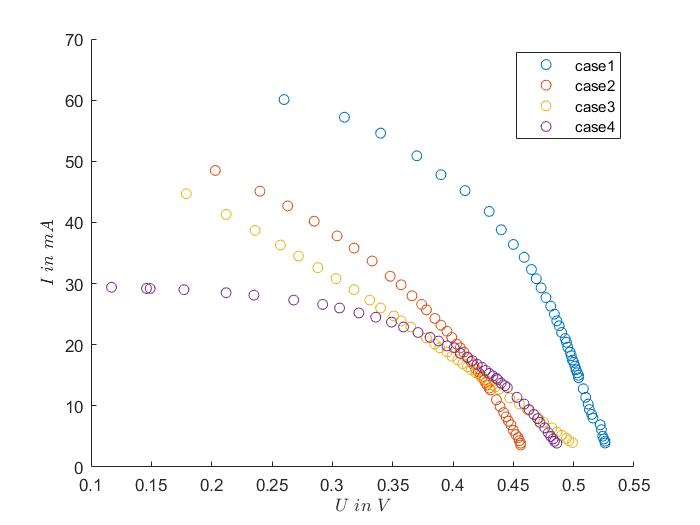
\includegraphics[scale=0.6]{Utot}\caption{the I-U curve for all 4 different measurements}\end{figure}

Out of these diagram and the measured data it becomes noticeable that we lack of parts of the curve, which are needed to determine all parameters. Therefore we have to fit those curves in order to get access to the missing curve parts. From the theory we know that the course of $I(U)$ follows the relation
\begin{equation*}I(U)=I_{ph}-I_0\left(\text{exp}\left(e\frac{U+R_s\,I}{n\,k_B\,T}\right)-1\right)-\frac{U+R_s\,I}{R_p}\end{equation*}
This is an equation, that first has to solved for I. Doing this I take advantage of the lambert w function, for which holds
\begin{equation*}z=x\,e^{x},\quad\text{only if }x=w(z)\end{equation*}
The starting equation can be reshaped as follows
\begin{gather*}\left(1+\frac{R_s}{R_p}\right)\,I=I_{ph}+I_0-\frac{U}{R_p}-I_0\,\text{exp}\left(e\frac{U+R_s\,I}{n\,k_B\,T}\right)\end{gather*}
In general it holds for
\begin{gather*}x=a-b\cdot{e}^{c\,x}\\(x-a)\,e^{-c\,x}=-b\\-c\cdot(x-a)\,e^{-c\,(x-a)}=c\,b\,e^{c\,a}\\\Rightarrow\;-c\,(x-a)=w\left(c\,b\,e^{c\,a}\right)\\
x=a-\frac{1}{c}\,w\left(c\,b\,e^{c\,a}\right)\end{gather*}
When we transfer this result to our particular case, $I$ can be written as
\begin{align*}I(U)=&\frac{I_{ph}+I_0}{1+\frac{R_s}{R_p}}-\frac{U}{R_p+R_s}\\
&-\frac{n\,k_B\,T}{e\,R_s}\,w\left(\frac{I_0}{1+\frac{R_s}{R_p}}\,\frac{e\,R_s}{n\,k_B\,T}\,\text{exp}\left(\frac{e\,U}{n\,k_B\,T}\right)\cdot\text{exp}\left(\frac{e\,R_s}{n\,k_B\,T}\cdot\left(\frac{I_{ph}+I_0}{1+\frac{R_s}{R_p}}-\frac{U}{R_p+R_s}\right)\right)\right)\end{align*}

where $R_s$ is the internal resistance in series $R_p$ is the internal parallel resistance and $n$ is a dimensionless factor. If we consider the cases 2 and 3, where additional resistance is applied, the equation doesn't change fundamentally. It only holds that the resistances transit to
\begin{equation*}R_s\;\rightarrow\;R_{s,0}+R_{s}'\end{equation*}
if an additional resistance in series is applied. And
\begin{equation*}R_p\;\rightarrow\;R_{p,0}+R_{p}'\end{equation*}
Therefore the form of the expression for the current stays the same.\newline
I approximated all 4 curves with a function of the form
\begin{equation*}I=a_1+a_2-a_3\,U-\frac{1}{a_4}\,w\left[a_4\,a_2\,\text{exp}(a_5\,U)\,\text{exp}\left(a_4\cdot(a_1+a_2-a_3\,U)\right)\right]\end{equation*}
and obtained following results.\newline\newline\newpage
The curve 1 could be approximated using the parameters\newline\newline
\begin{tabular}{ccccc}$a_1=81.6695$&$a_2=1.8\cdot10^{-7}$&$a_3=80.7537$&$a_4=0.0399$&$a_5=35.9712$\end{tabular}
\begin{figure}[H]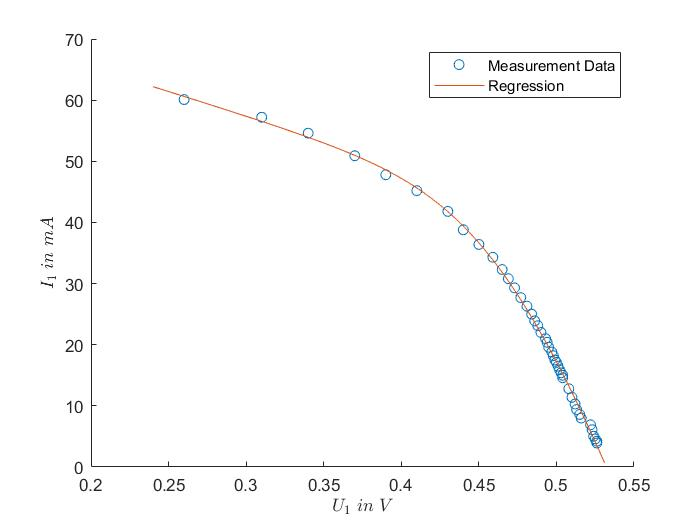
\includegraphics[scale=0.4]{gef. KL 1}\caption{the course of the measured points of the first I-U curve with a regression}\end{figure}
for the 2. measurement I obtained\newline\newline
\begin{tabular}{ccccc}$a_1=63.933$&$a_2=0.246$&$a_3=66.525$&$a_4=1.7\cdot10^{-5}$&$a_5=10.528$\end{tabular}
\begin{figure}[H]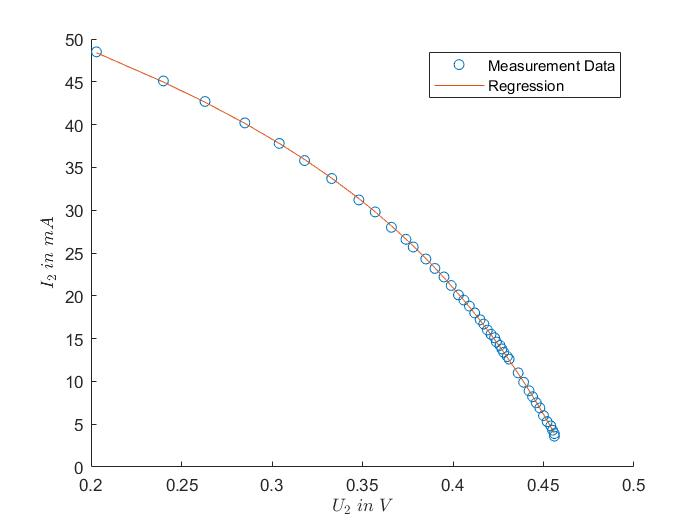
\includegraphics[scale=0.4]{gef. KL 2}\caption{the course of the measured points of the 2. I-U curve with a regression}\end{figure}\newpage
for the 3. case the following parameters were found\newline\newline
\begin{tabular}{ccccc}$a_1=137.136$&$a_2=46.036$&$a_3=2.7\cdot10^{-4}$&$a_4=0.014$&$a_5=2.595$\end{tabular}
\begin{figure}[H]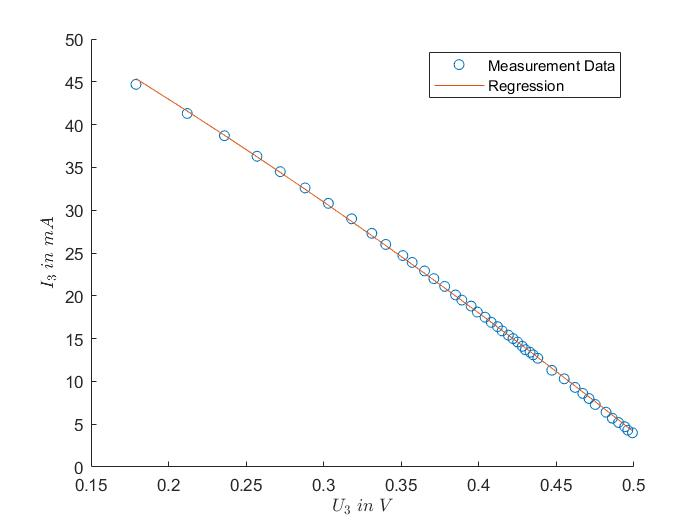
\includegraphics[scale=0.4]{gef. KL 3}\caption{the course of the measured points of the 3. I-U curve with a regression}\end{figure}
and finally for the 4. data set these results were found\newline\newline
\begin{tabular}{ccccc}$a_1=29.93$&$a_2=0.172$&$a_3=0.035$&$a_4=8.3\cdot10^{-6}$&$a_5=10.354$\end{tabular}
\begin{figure}[H]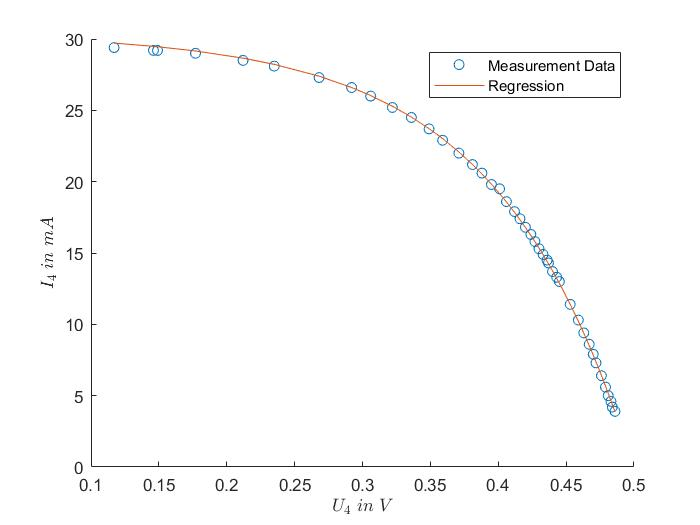
\includegraphics[scale=0.4]{gef. KL 4}\caption{the course of the measured points of the 4. I-U curve with a regression}\end{figure}
\newpage
Using the relation $P=I\cdot{U}$ we can depict the course of the power in dependence of the voltage.
\begin{figure}[H]\centering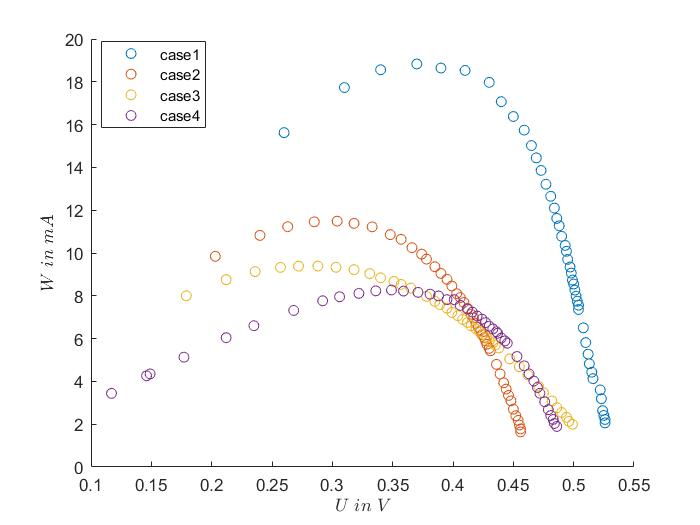
\includegraphics[scale=0.7]{Ptot}\caption{the course of the power for all four different measurements}\end{figure}

\newpage
In the following the power curves along with the curves obtained the fit functions from above are shown.
\begin{figure}[H]\centering
\begin{adjustwidth}{-1em}{7em}
  \begin{subfigure}[b]{0.5\textwidth}
    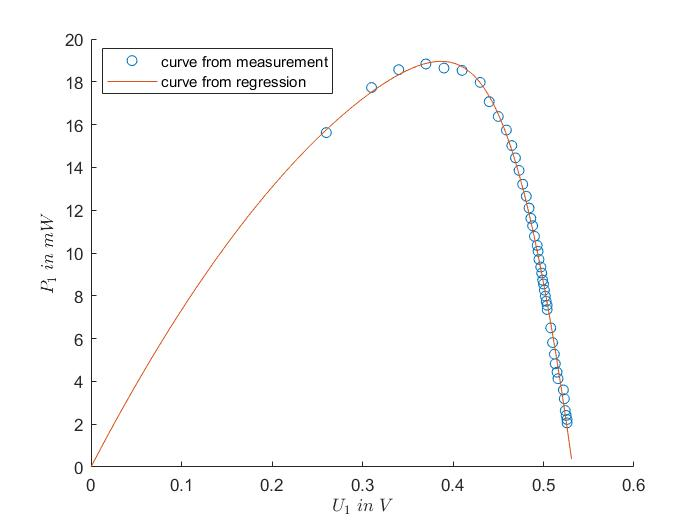
\includegraphics[width=\textwidth]{P1}
    \caption{power curve 1}
    \label{fig:}
  \end{subfigure}
  %
  \begin{subfigure}[b]{0.5\textwidth}
    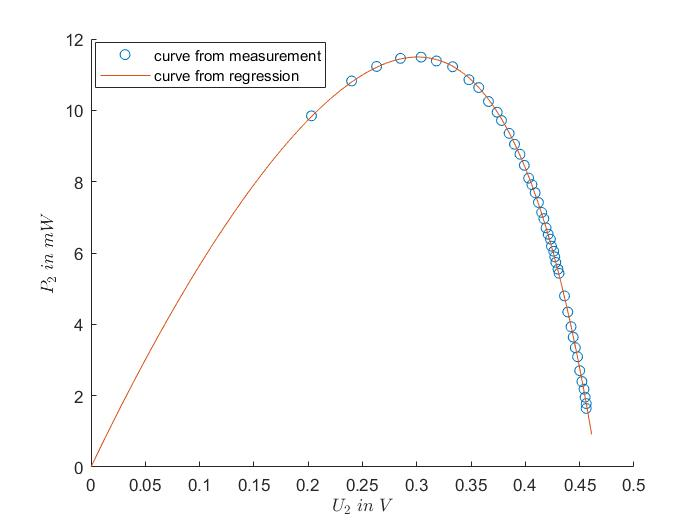
\includegraphics[width=\textwidth]{P2}
    \caption{power curve 2}
    \label{fig:}
  \end{subfigure}
\end{adjustwidth}\centering
\begin{adjustwidth}{-1em}{7em}
  \begin{subfigure}[b]{0.5\textwidth}
    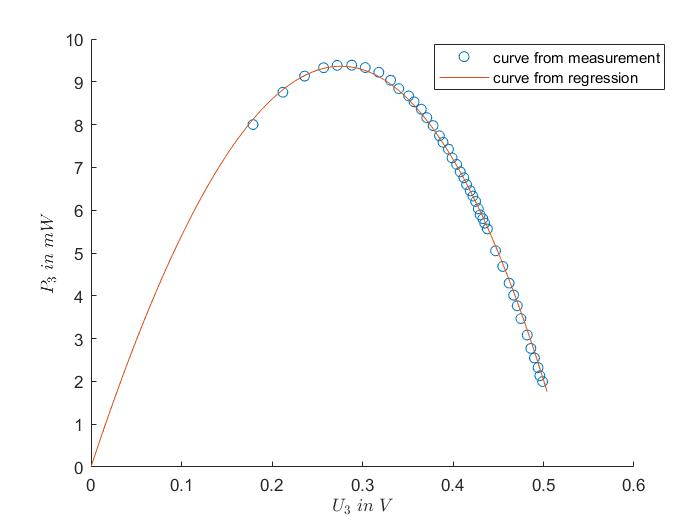
\includegraphics[width=\textwidth]{P3}
    \caption{power curve 3}
    \label{fig:}
  \end{subfigure}
  %
  \begin{subfigure}[b]{0.5\textwidth}
    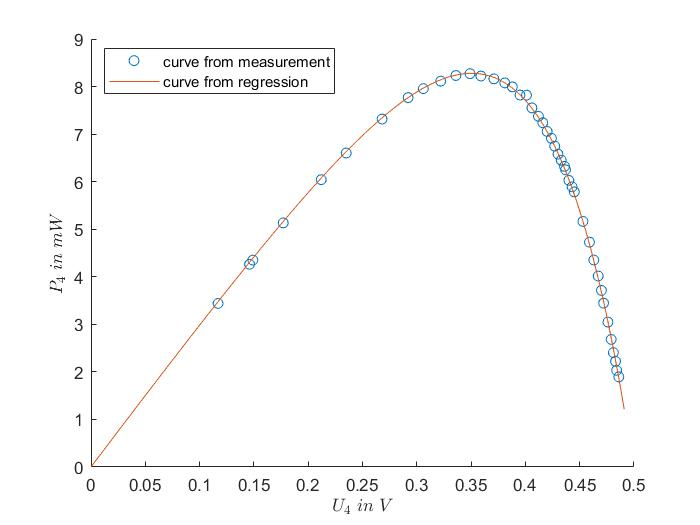
\includegraphics[width=\textwidth]{P4}
    \caption{power curve 4}
    \label{fig:}
  \end{subfigure}
\end{adjustwidth}
\caption{the the power curves of the different measurement with the power curves using the parameters of the previous fits}
\end{figure}







Using the regression functions, I calculated the characteristics of the different settings of each case, which are collected in the following table. We measured the irradiated area of the solar cell to 78 $\text{mm}^2$ and the illumination intensity to $E_v=27000$ lux for the first three measurements and $E_v=102500$ lux for the fourth measurement. \newline
This values where were converted into irradiance intensity $E_e$ by using the special luminous efficacy $K=E_v/E_e\approx300\,lm/W$. For the calculation of $I_{sc}$ and $U_{oc}$ I used the relations $I_{sc}=I(U=0)$ and $V_{oc}=U(I=0)$.

\begin{table}[H]\begin{tabular}{c || c ||c  ccccccc}\multirow[c]{2}{*}{case}&\multirow[c]{2}{2cm}{measurement}&\multirow[c]{2}{1cm}{$E_e$\newline($W/m^2$)}&\multirow[c]{2}{1cm}{$I_{sc}$\newline(mA)}&\multirow[c]{2}{1cm}{$V_{oc}$\newline(V)}&\multirow[c]{2}{1cm}{$P_{MPP}$\newline(mW)}&\multirow[c]{2}{1cm}{FF\newline(\%)}&\multirow[c]{2}{1cm}{$\eta$\newline(\%)}&\multirow[c]{2}{1cm}{$R_p$\newline($\Omega$)}&\multirow[c]{2}{1cm}{$R_s$\newline($\Omega$)}\\&&&&&&&&&\\\hline\hline
1&\multirow[c]{1}{2.5cm}{$I_{sc}=60\,mA$}&900&81.669&0.532&18.943&43.579&26.985&12.383&1.728\\&&&&&&&&&\\
2&\multirow[c]{1}{2.5cm}{$I_{sc}=60\,mA\;\newline{R}_p=15\,\Omega$}&900&63.932&0.466&11.526&38.709&16.419&14.467&2.405\\&&&&&&&&&\\
3&\multirow[c]{1}{2.5cm}{$I_{sc}=60\,mA\;\newline{R}_s=5.1\,\Omega$}&900&67.802&0.532&9.37&25.971&13.348&8.561&7.325\\&&&&&&&&&\\
4&\multirow[c]{1}{2.5cm}{$I_{sc}=30\,mA$}&341.667&29.93&0.499&8.282&55.442&31.076&552.323&3.211\end{tabular}\caption{the results of the evaluation using the fit parameters}\end{table}

We can observe that the short cut current and the open circle voltage are less influenced by the additional connection of the parallel resistance than 0f the serial resistance, but the efficiency drops more when the serial resistance is linked up than for the parallel pendant. We can now test our fit solution on how consistent it relates the resistances. It should hold
\begin{equation*}R_{p,2}\overset{!}{=}R_{p,2}'\coloneqq\left(\frac{1}{R_{p,1}}+\frac{1}{15\,\Omega}\right)^{-1}\end{equation*}
But the result for $R_{p,2}'=6.783\,\Omega$, whereas $R_{p,2}=14.467\,\Omega$. This is quite far away from the reality. For the serial resistance the results are better. \newline
The difference $\Delta{R_s}\coloneqq{R_{s,3}-R_{s,1}}=5.597\,\Omega$, while it should be the $5.1\,\Omega$ from the additional serial resistance. The situation that, the approximation for $R_s$ seems to be far better than for $R_p$, can probably be explained by considering, that the measured data points are way closer to the x-axis cross section than to the y-axis cross section. Therefore the regression should be better in this part of the I-U curve.
This might explain, too, why the resistance $R_{p,4}$ with $552\,\Omega$ seems to be completely out of range, whereas it should be the same as for case 1.\newline\newline
The values for the efficiency can be assessed as quite good, because the values could have been taken from the measured data directly, and therefore have been calculated from a part of the regression which fitted very well to the data. \newline\newline
In the end I want to examine the effect of the temperature on the I-U curve and the characteristics of the solar cell. I proceed that by running a matlab simulation, which was provided to us by the university. With a chosen short cut current of 60 mA I examine the effect of the temperature by evaluating the I-U curves for the 25°C, -15°C and 40°C.
\begin{figure}[H]\centering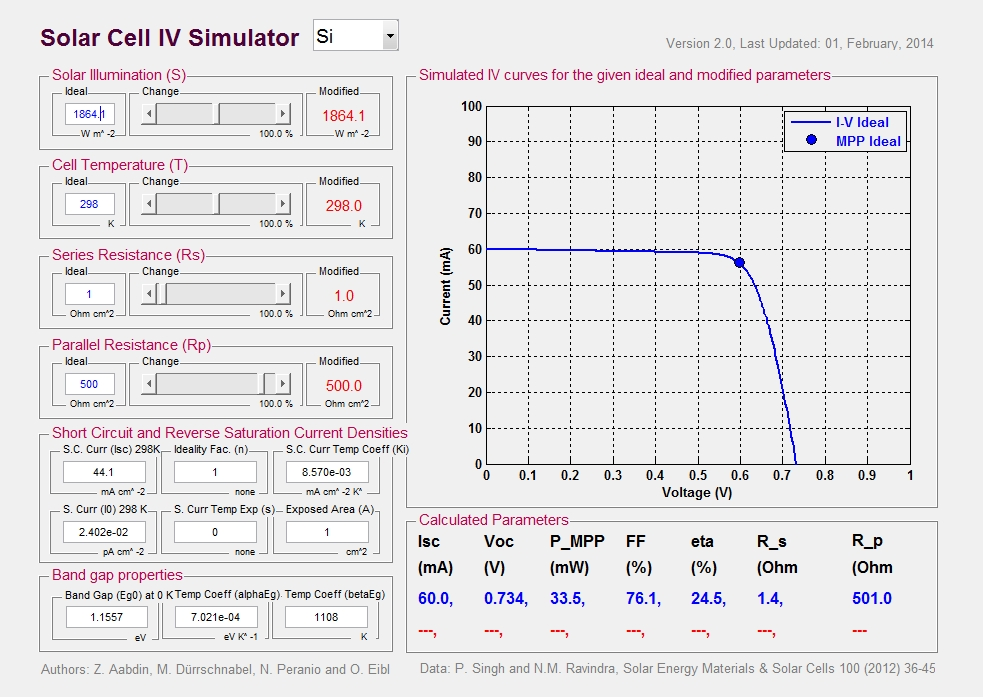
\includegraphics[scale=0.4]{25 degree}\caption{The simulation of the I-U curve for 25°C}\end{figure}

\begin{figure}[H]\centering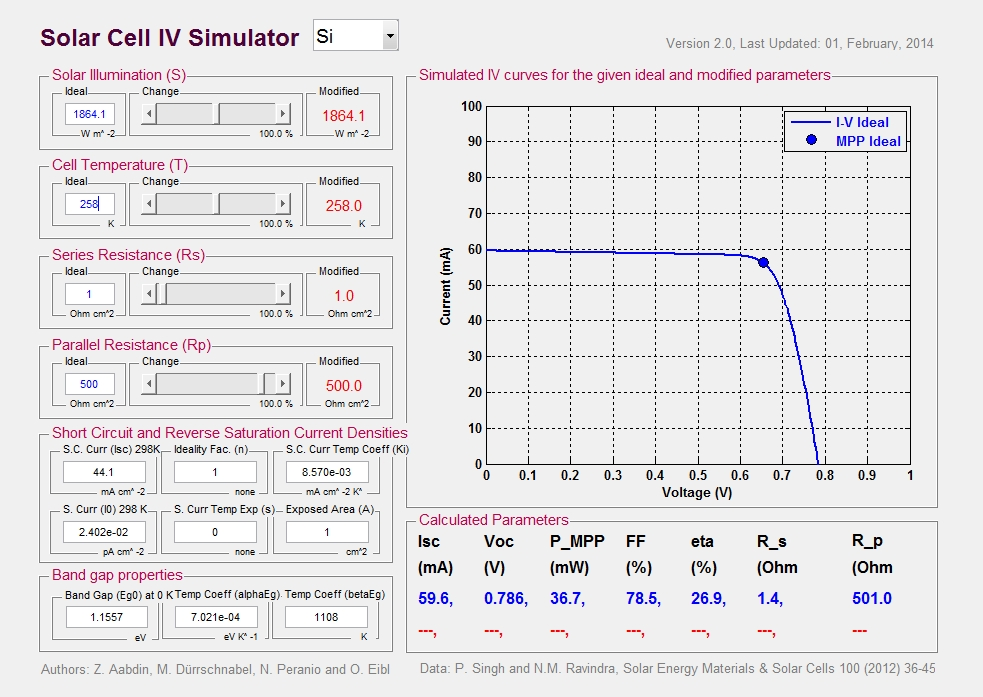
\includegraphics[scale=0.4]{-15 degree}\caption{The simulation of the I-U curve for -15°C}\end{figure}

\begin{figure}[H]\centering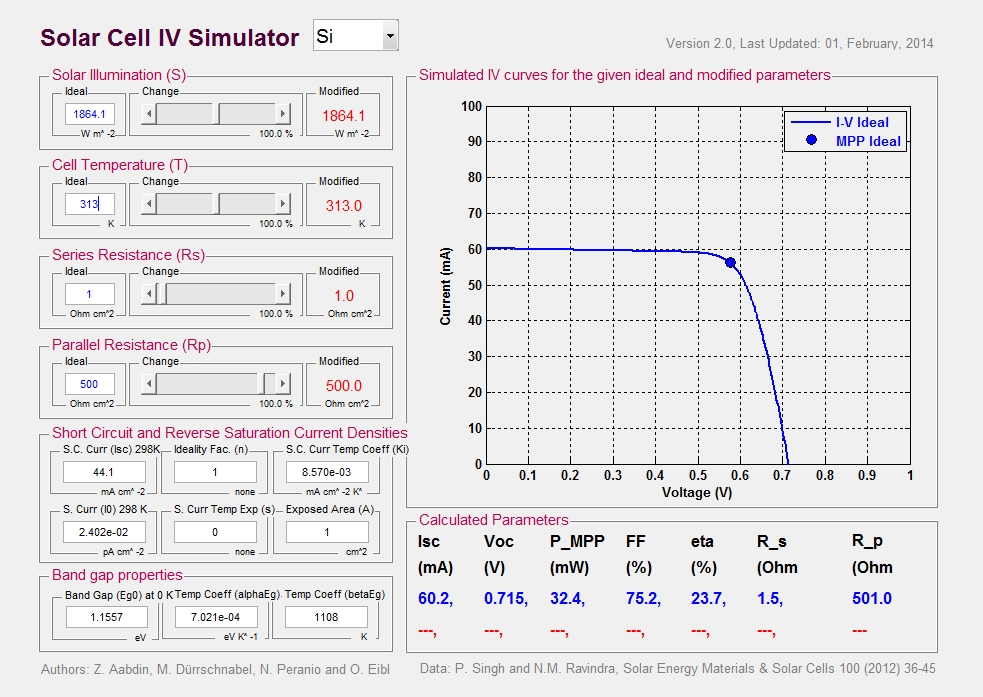
\includegraphics[scale=0.4]{40 degree}\caption{The simulation of the I-U curve for 40°C}\end{figure}

\begin{table}[H]\centering\begin{tabular}{|c | c |c | c |c |c|}\hline
\multirow[c]{2}{*}{temperature}&\multirow[c]{2}{1cm}{$I_{sc}$\newline(mA)}&\multirow[c]{2}{1cm}{$V_{oc}$\newline(V)}&\multirow[c]{2}{1cm}{$P_{MPP}$\newline(mW)}&\multirow[c]{2}{1cm}{FF\newline(\%)}&\multirow[c]{2}{1cm}{$\eta$\newline(\%)}\\
&&&&&\\\hline\hline
-15°C&59.6&0.786&36.7&78.5&26.9\\\hline
25°C&60&0.734&33.5&76.1&24.5\\\hline
40°C&60.2&0.715&32.4&75.2&23.7\\\hline
\end{tabular}\caption{results of the simulation with respect to the temperature}\end{table}
It can be assessed that the maximum power as well as the efficiency decrease with increasing temperature. This fact is in some extend of course counter productive to the practical application.
\newpage
\section{Conclusion}
With the measurement results we can only partly be satisfied. The I-U curves and the P-U curves of the measured data showed a nice course, but especially for the I-U curves the measurement range was a little bit to small to get really good results for the parallel resistance. Despite that our results for the maximum Power and efficiency were good and valid. Because this are the most important values of the solar cell, we have been never the less capable to characterize our solar cell quite aptly. By also taking a look at the simulations for the effect of the temperature, we could further understand some of the difficulties that occur, when using solar cells in practice.















\end{document}










